%solucion del problema numero 5 con las 6 D's


\subsection{Descripción del problema}
Dado un numero binario de $n$ bits regresar su equivalente en decimal.


\begin {figure}[h!]
\centerline{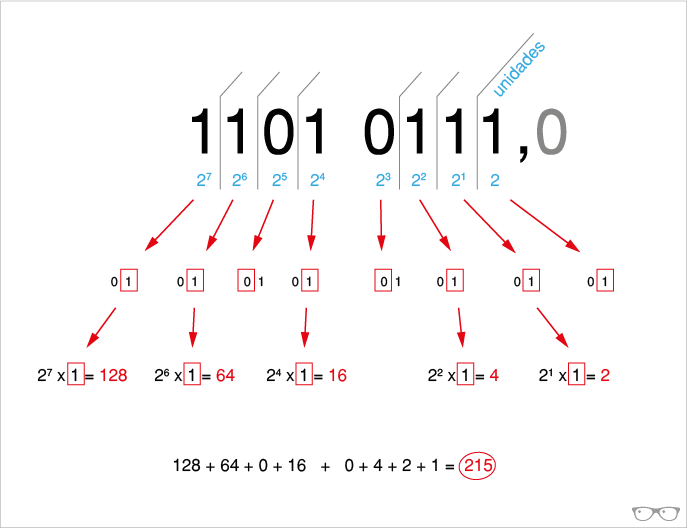
\includegraphics[width = 6cm ]{Latex-imágenes/conversion-binario-decimal.png}}
\caption{Conversión binario-decimal}
\label{fig}
\end {figure}

\subsection{Definición de la solución}
El proceso de conversión de un número binario a decimal se realiza de la siguiente manera: se enumeran los dígitos de derecha a izquierda, comenzando desde la posición cero. Se utiliza como base el número 2 y se suma el valor correspondiente a cada posición. Es decir, se eleva la base (2) al exponente de la posición en la que se encuentra el dígito, pero solo se realiza la suma si en esa posición hay un 1. Si se encuentra un 0, no se realiza ninguna suma.

\subsection{Diseño de la solución}

\begin {figure}[h!]
\centerline{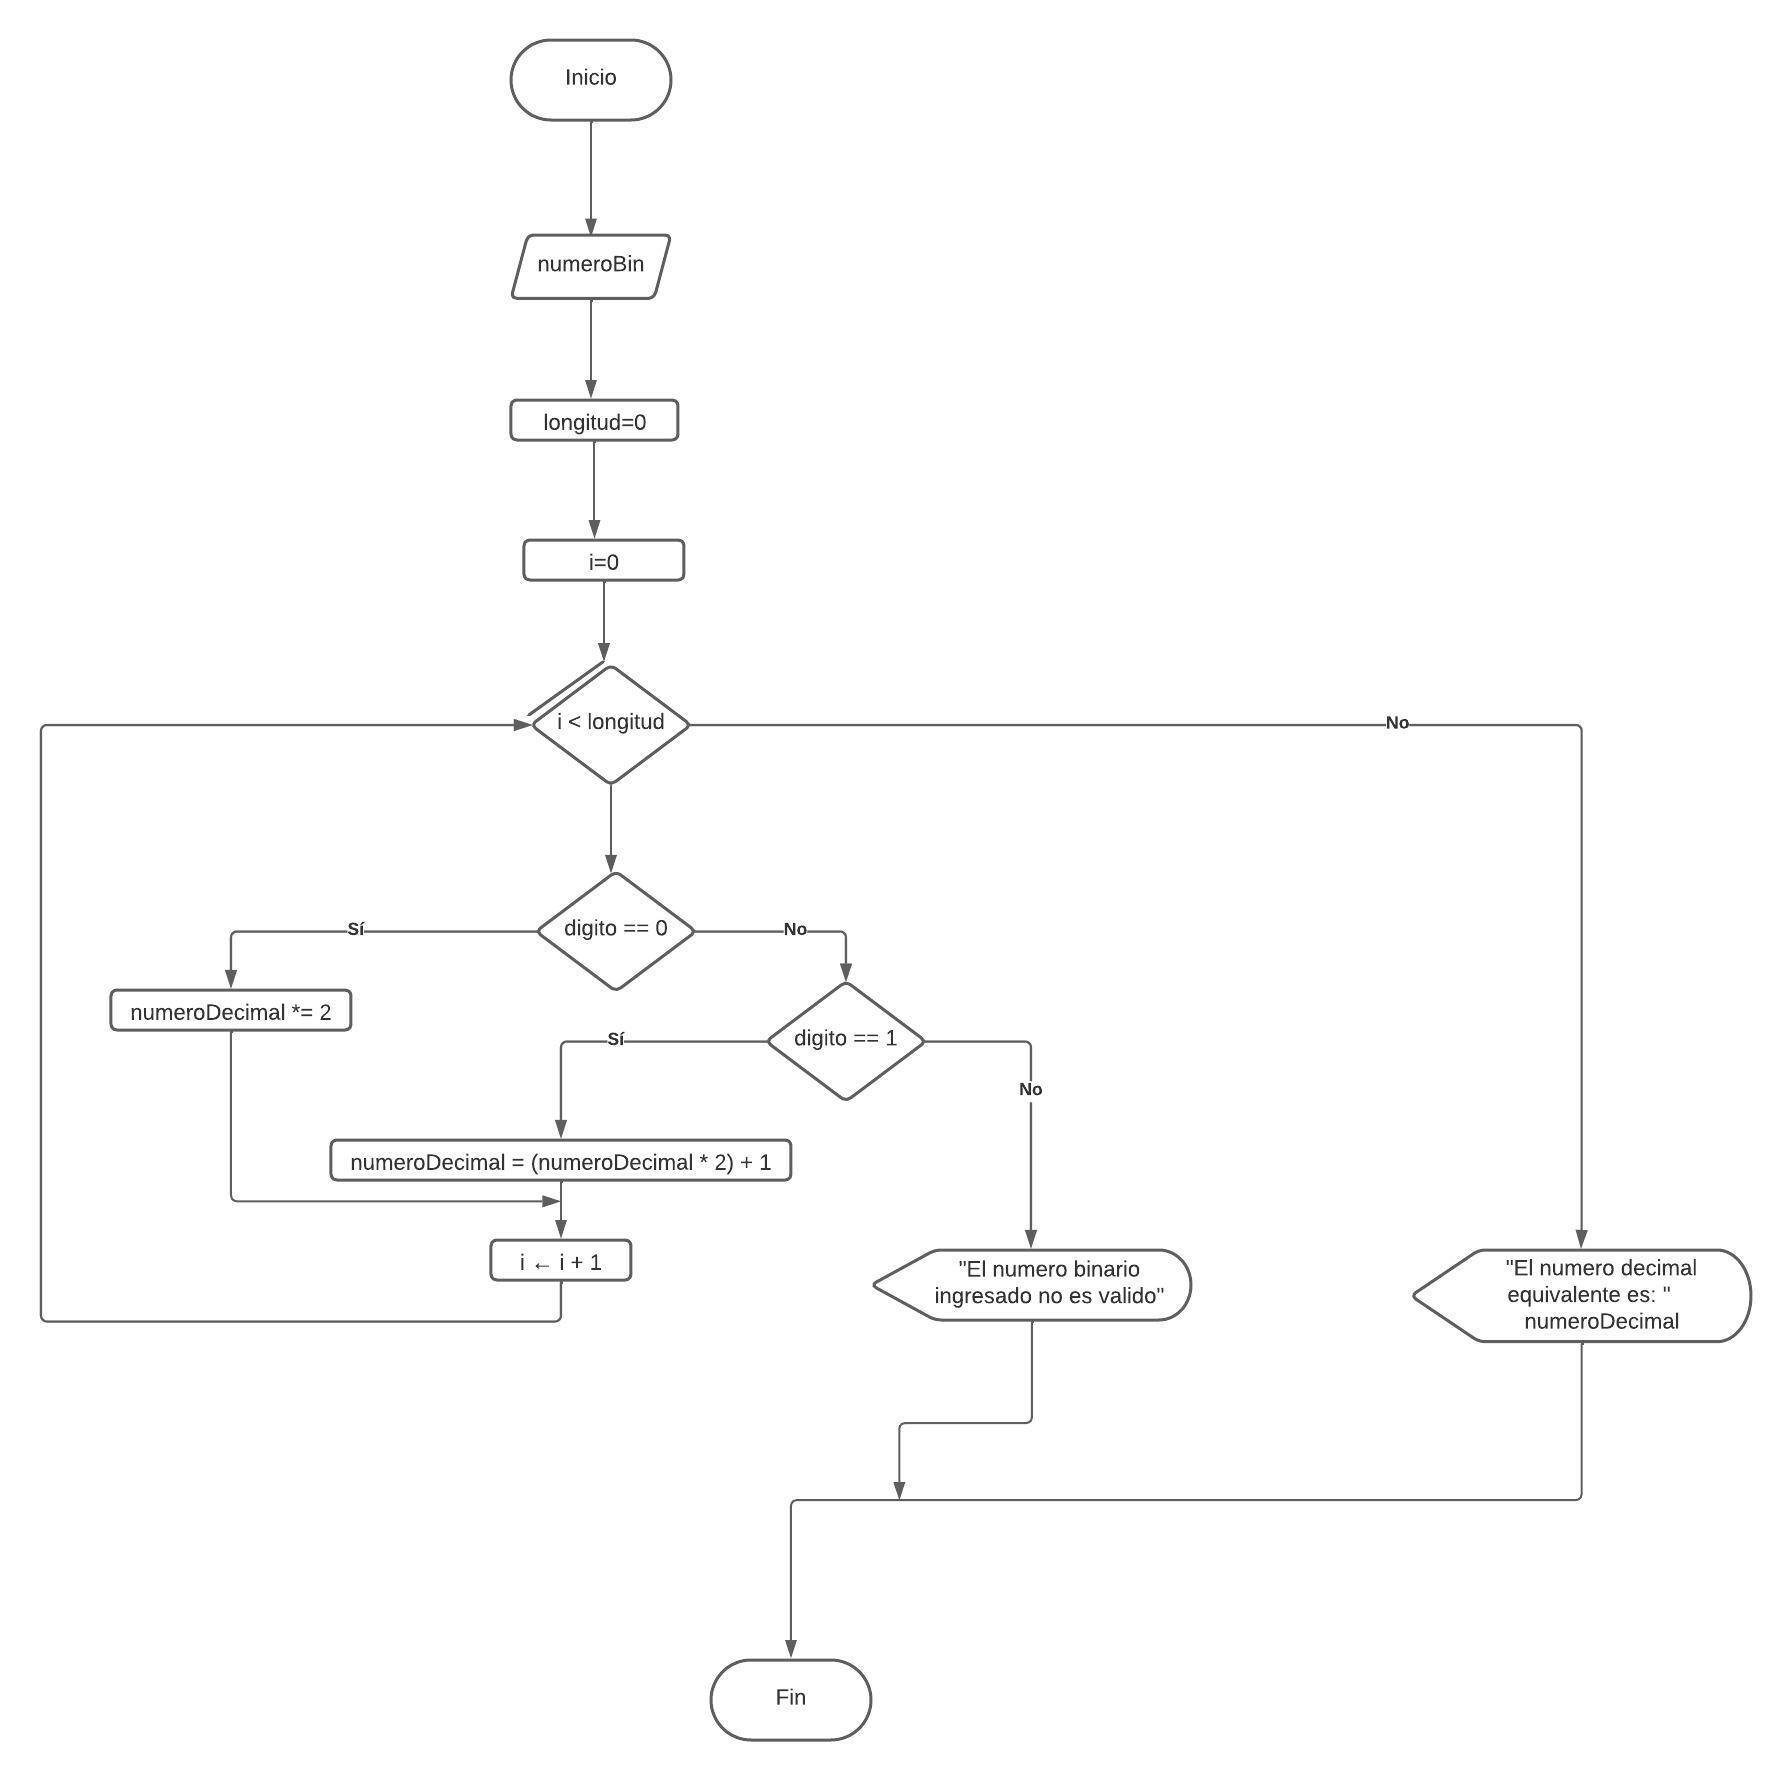
\includegraphics[width = 6cm]{Latex-imágenes/diagramaEx5.jpeg}}
\caption{Diagrama de flujo del problema 4}
\label{fig}
\end {figure}



\subsection{Desarrollo de la solución}

En el siguiente bloque de código, se muestra una ventana flotante que pide al usuario que ingrese un numero binario 

\begin{javaCode}
    String numeroBin = JOptionPane.showInputDialog("Ingresa un numero binario");
        int longitud = numeroBin.length();
        int numeroDecimal = 0;
\end{javaCode}

Después se toma ese numero y se compara si solo contiene ceros y unos, si es así el código hace las respectivas operaciones para poder obtener el numero decimal y en dado caso que el numero ingresado contenga algo mas que ceros y unos se mostrara el mensaje: " El numero binario ingresado no es valido"

\begin{javaCode}
        for (int i = 0; i < longitud; i++) {
            
            char digito = numeroBin.charAt(i);
            
            if (digito == '0') {
                numeroDecimal *= 2;
            } else if(digito == '1') {
                numeroDecimal = (numeroDecimal * 2) + 1;
            } else {
                JOptionPane.showMessageDialog(null, "El numero binario ingresado no es valido");
                return;
            }
        }
\end{javaCode}

Por ultimo si el numero ingresado solo contiene ceros y unos se muestra una ventana flotante con el resultado de la convección binario-decimal

\begin{javaCode}
JOptionPane.showMessageDialog(null, "El numero decimal equivalente es " + numeroDecimal);
\end{javaCode}

\subsection{Depuración de pruebas}

La siguiente tabla muestra el resultado de la compilación del codigo
\begin{table}[h!]
  \centering
  \caption{Tabla de corridas para el Ejercicio 5.}
  \label{tab:tabla_ejemplo}
  \begin{tabular}{|l|c|r|}
    \hline
    \textbf{$Binario$} & \textbf{Decimal} \\
    \hline
    111 & 7 \\
    10101010 & 170 \\
    675 & " El numero binario ingresado no es valido" \\
    110101 & 53 \\
    2 & " El numero binario ingresado no es valido" \\
    
    \hline
  \end{tabular}
\end{table}